% Created 2017-05-14 Sun 09:03
% Intended LaTeX compiler: pdflatex
\documentclass[a4paper,11pt]{article}
\usepackage[utf8]{inputenc}
\usepackage[T1]{fontenc}
\usepackage{graphicx}
\usepackage{grffile}
\usepackage{longtable}
\usepackage{wrapfig}
\usepackage{rotating}
\usepackage[normalem]{ulem}
\usepackage{amsmath}
\usepackage{textcomp}
\usepackage{amssymb}
\usepackage{capt-of}
\usepackage{hyperref}
\usepackage[margin=1.2in]{geometry}
\usepackage{setspace}
\onehalfspacing
\usepackage{parskip}
\usepackage{amsthm}
\usepackage{amsmath}
\usepackage{mathtools}
\usepackage{hyperref}
\usepackage{graphicx}
\usepackage{tabularx}
\usepackage{booktabs}
\usepackage{color}
\usepackage{caption}
\usepackage{subcaption}
\hypersetup{colorlinks,citecolor=black,filecolor=black,linkcolor=black,urlcolor=black}
\newtheorem{mydef}{Definition}
\newtheorem{mythm}{Theorem}
\newcommand{\dx}{\mathrm{d}}
\newcommand{\var}{\mathrm{Var}}
\newcommand{\cov}{\mathrm{Cov}}
\newcommand{\corr}{\mathrm{Corr}}
\newcommand{\pr}{\mathrm{Pr}}
\newcommand{\rarrowd}[1]{\xrightarrow{\text{ \textit #1 }}}
\DeclareMathOperator*{\plim}{plim}
\newcommand{\plimn}{\plim_{n \rightarrow \infty}}
\setcounter{secnumdepth}{2}
\author{Zheng Tian}
\date{}
\title{Lecture 10: Nonlinear Regression Functions}
\hypersetup{
 pdfauthor={Zheng Tian},
 pdftitle={Lecture 10: Nonlinear Regression Functions},
 pdfkeywords={},
 pdfsubject={},
 pdfcreator={Emacs 25.1.1 (Org mode 9.0.3)}, 
 pdflang={English}}
\begin{document}

\maketitle

\section{Introduction}
\label{sec:org3b81277}
\subsection{Overview}
\label{sec:org54f5667}
In the previous lectures, the population regression function is
assumed to be linear. In other words, the slope of the population
regression function was constant, so the effect on Y of a unit change
in X does not itself depend on the value of X, neither on other
independent variables. In some cases, the linearity cannot capture the
feature of the data and may also contradict with economic theories or
common sense.

This lecture introduces nonlinear population regression
functions that are nonlinear with respect to
the regressors but linear with respect to the parameters. Such
regression models can still be considered as being "linear" due to the
linearity in the parameters so that they can be estimated using the
OLS method we have known. Specifically, we will introduce three types
of nonlinear regression functions, the polynomial function, the
logarithmic function, and the function with the interaction terms
consisting of two independent variables.

Since these types of models can be estimated using the OLS, the
estimation and inference are not the foci of this lecture. Instead, we
put emphasis on the correct interpretation of the coefficients in each
type of models.

\subsection{Reading materials}
\label{sec:org50e7d4a}
\begin{itemize}
\item Chapter 8 in \emph{Introduction to Econometrics} by Stock and Watson.
\end{itemize}


\section{A General Strategy For Modeling Nonlinear Regression Functions}
\label{sec:org2df2f97}

\subsection{Test Scores and district income}
\label{sec:org429408f}

In the application of California elementary schools, we know that test
scores can be determined by average district income, along with
student-teacher ratios that we have included in regression. For
simplicity, let's just consider the relationship between test scores
and district income using a scatterplot. As shown in Figure
\ref{fig:org7c2cdc1}, test scores and district income are indeed
positively correlated, with a correlation coefficient of 0.71.

\begin{figure}[htbp]
\centering
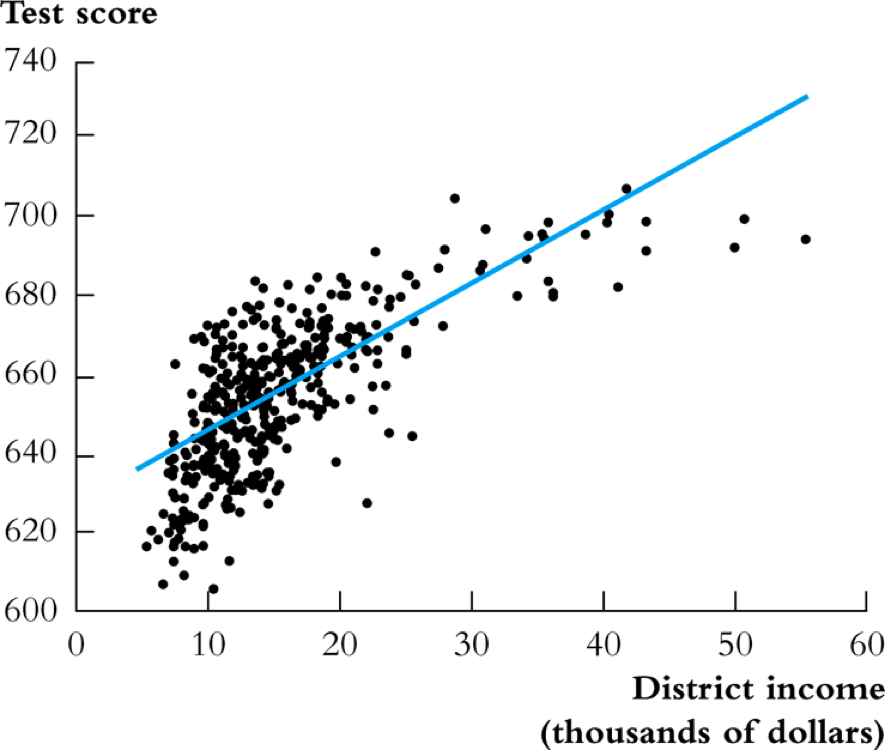
\includegraphics[width=0.75\textwidth]{img/fig-8-2.png}
\caption{\label{fig:org7c2cdc1}
Scatterplot of test score vs district income and a linear regression line}
\end{figure}

\subsubsection*{How does a simple linear regression model fit the data?}
\label{sec:org44b354c}

We estimate a simple linear regression model
\[TestScore = \beta_0 + \beta_1 Income + u\]

The sample regression line is superimposed on the
scatterplot. However, we can observe some problems of using the linear
regression line to fit the data

\begin{itemize}
\item Data points are below the regression line when income is very
low (under \$10,000) or very high (over \$40,000), and are above the
line when income is between \$15,000 and \$30,000.
\item The scatterplot may imply a curvature in the relationship between
test scores and income. That is, a unit increase in income may have
larger effect on test scores when income is very low than when
income is very high.
\item The linear regression line cannot capture the curvature because the
effect of district income on test scores is constant over all the
range of income since \(\Delta TestScore / \Delta Income = \beta_1\)
is constant.
\end{itemize}

\subsubsection*{Estimate a quadratic regression model}
\label{sec:org885e0ac}

Instead of estimating a linear regression model, we can set up a
quadratic regression model as
\begin{equation}
\label{eq:quadratic-testscore}
TestScore = \beta_0 + \beta_1 Income + \beta_2 Income^2 + u
\end{equation}

\begin{itemize}
\item This model is nonlinear, specifically quadratic, with respect to
\(Income\) because we include the squared income.
\item The population regression function is
\[E(TestScore | Income) = \beta_0 + \beta_1 Income + \beta_2 Income^2\]
\item But it is linear with respect to \(\beta\). So we can still use the
OLS estimation method to estimate the model, and use \(R^2\), t and F
statistics for inference as we do in multiple regression. We simply
treat \(Income^2\) as another regressor in a multiple regression model.
\item The quadratic regression line is added onto the scatterplot, which
fits the points better than the linear regression line, as shown in
Figure \ref{fig:org3cb8574}.

\begin{figure}[htbp]
\centering
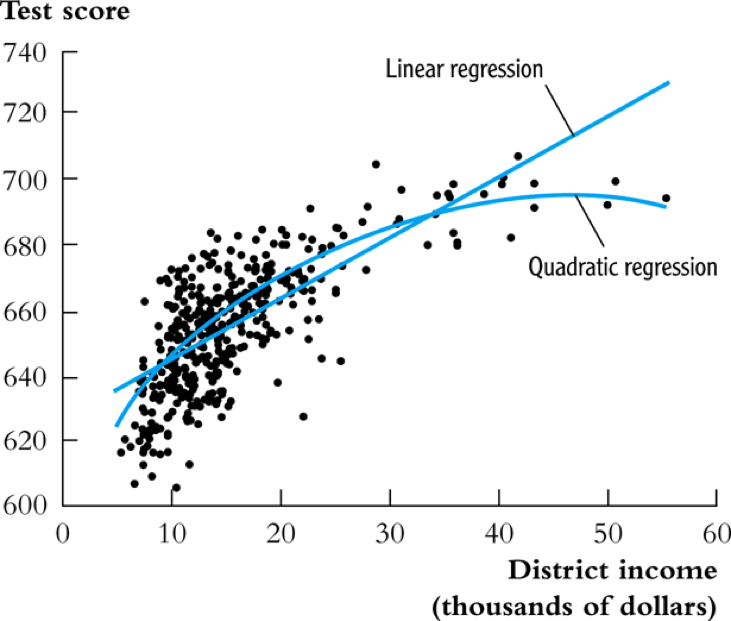
\includegraphics[width=0.75\textwidth]{img/fig-8-3.png}
\caption{\label{fig:org3cb8574}
Scatterplot of test score vs district income and a quadratic regression line}
\end{figure}
\end{itemize}


\subsection{A general formula for a nonlinear population regression function}
\label{sec:org43f5afe}

A general nonlinear regression model is
\begin{equation}
\label{eq:nl-general}
Y_i = f(X_{i1}, X_{i2}, \ldots, X_{ik}; \beta_1, \beta_2, \ldots, \beta_m) + u_i
\end{equation}

where \(f(X_{i1}, X_{i2}, \ldots, X_{ik}; \beta_1, \beta_2, \ldots,
\beta_m)\) is the \textbf{population nonlinear regression function}. Note that
the number of regressors and the number of parameters are not
necessarily equal in the nonlinear regression model.

We can use \(\mathbf{X}_i = (X_{i1}, \ldots, X_{ik})\) to represent all
regressors for the i\(^{\text{th}}\) observation, and use
\(\boldsymbol{\beta}=(\beta_1, \beta_2, \ldots, \beta_m)\) to represent
the parameters to be estimated. Then, the nonlinear regression model
in Equation (\ref{eq:nl-general}) can be re-written as

\begin{equation}
\label{eq:nl-general-mat}
Y_i = f(\mathbf{X}_i; \boldsymbol{\beta}) + u_i
\end{equation}

In this lecture, we focus on the nonlinear regression models
such that \(f(\cdot)\) is nonlinear with \(\mathbf{X}_i\) but linear with
\(\boldsymbol{\beta}\). So this type of models are also consider as
being "linear" and estimated by the OLS method.


\subsection{The effect on \(Y\) of a change in a regressor}
\label{sec:orga1190ca}

For the general nonlinear model in Equation (\ref{eq:nl-general}), the
effect on \(Y\) of a change in one regressor, say \(X_1\), holding other
things constant, can be computed as
\begin{equation}
\label{eq:nl-gen-effect}
\Delta Y = f(X_1 + \Delta X_1, X_2, \ldots, X_k; \boldsymbol{\beta}) - f(X_1, X_2, \ldots, X_k; \boldsymbol{\beta})
\end{equation}
When \(X_1\) and \(Y\) are continuous variables and \(f(\cdot)\) is
differentiable, the marginal effect of \(X_1\) is the partial derivative
of \(f\) with respect to \(X_1\), that is, holding other things constant

\[ \Delta Y = \frac{\partial f(X_1, \ldots, X_k; \boldsymbol{\beta})}{\partial X_1} \Delta X_1  \]


\subsection{Application to test scores and income}
\label{sec:orgae6b48d}

We estimate the quadratic regression model for test scores and
district income (Equation \ref{eq:quadratic-testscore}) by OLS,
resulting in the following

\begin{equation}
\label{eq:tsr-income2}
\widehat{TestScore} = \underset{\displaystyle (2.9)}{607.3} +
\underset{\displaystyle (0.27)}{3.85}Income - \underset{\displaystyle (0.0048)}{0.0423}Income^2,\, \bar{R}^2 = 0.554
\end{equation}


We can test whether the squared income has a significant
coefficient. That is, we test \(H_0:\, \beta_2 = 0 \text{ vs. } H_1:\,
\beta_2 \neq 0\). In other words, we test the quadratic regression mode
against the linear regression model. For this two-sided test, we can
as usual compute the t-statistic

\[ t = \frac{-0.0423}{0.0048} = -8.81 > -1.96 \]

Thus, we can reject the null at the 1\%, 5\% and 10\% significance levels.

From Equation (\ref{eq:tsr-income2}), we can compute the effect of
change in district average income on test scores.
\subsubsection*{A change in income from \$10 thousand to \$20 thousand}
\label{sec:org6fd9759}
\begin{equation*}
\begin{split}
\Delta \hat{Y} &= \hat{\beta}_0 + \hat{\beta}_1 \times 11 + \hat{\beta}_2 \times 11^2 - (\hat{\beta}_0 + \hat{\beta}_1 \times 10 + \hat{\beta}_2 \times 10^2) \\
&= \hat{\beta}_1 (11 - 10) + \hat{\beta}_2(11^2 - 10^2) \\
& = 3.85 - 0.0423 \times 21 = 2.96
\end{split}
\end{equation*}
Thus, the predicted difference in test scores between a district with
average income of \$11,000 and one with average income of \$10,000 is
2.96 points.

\subsubsection*{A change in income from \$40 thousand to \$41 thousand}
\label{sec:org7107981}
\begin{equation*}
\begin{split}
\Delta \hat{Y} &= \hat{\beta}_0 + \hat{\beta}_1 \times 41 + \hat{\beta}_2 \times 41^2 - (\hat{\beta}_0 + \hat{\beta}_1 \times 40 + \hat{\beta}_2 \times 40^2) \\
&= \hat{\beta}_1 (41 - 40) + \hat{\beta}_2(41^2 - 40^2) \\
& = 3.85 - 0.0423 \times 81 = 0.42
\end{split}
\end{equation*}
Thus, the predicted difference in test scores between a district with
average income of \$41,000 and one with average income of \$40,000 is
0.42 points. Thus, a change of income of \$1,000 is associated with a
larger change in predicted test scores if the initial income is
\$10,000 than if it is \$40,000.


\subsection{A general approach to modeling nonlinearities using multiple regression}
\label{sec:orga2accc6}
\begin{enumerate}
\item Identify a possible nonlinear relationship.
\begin{itemize}
\item Economic theory
\item Scatterplots
\item Your judgment and experts' opinions
\end{itemize}
\item Specify a nonlinear function and estimate its parameters by OLS.
\begin{itemize}
\item The OLS estimation and inference techniques can be used as usual
when the regression function is linear with respect to \(\beta\).
\end{itemize}
\item Determine whether the nonlinear model improves upon a linear model
\begin{itemize}
\item Use t- and/or F-statistics to test the null hypothesis that the
population regression function is linear against the alternative
that it is nonlinear.
\end{itemize}
\item Plot the estimated nonlinear regression function.
\item Compute the effect on \emph{Y} of a change in \emph{X}.
\end{enumerate}
\end{document}